\section{Analityczny model projektowy dziedziny}
\begin{figure}[h!]
	\centering
	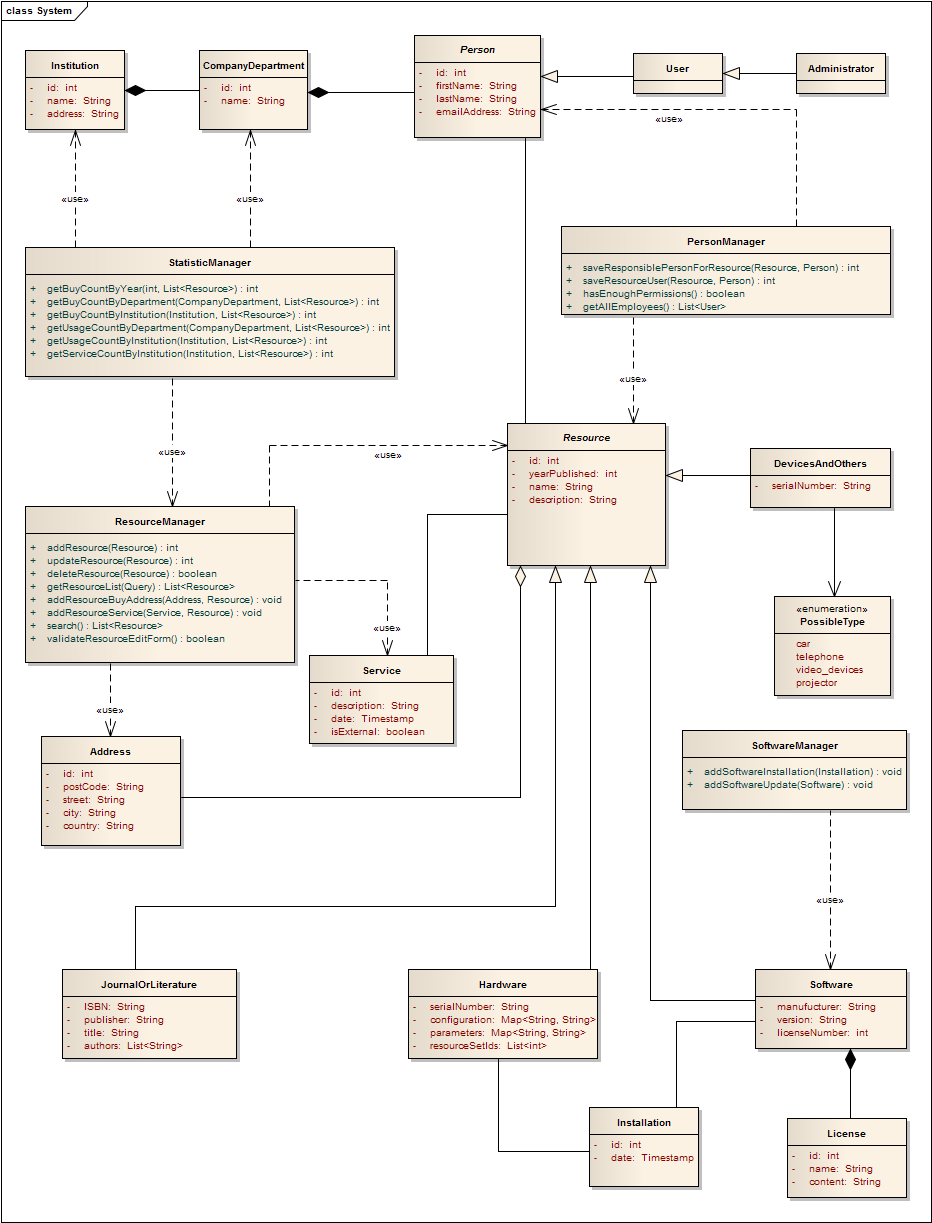
\includegraphics[scale=0.4]{img/class-diagram2}
	\caption{Diagram klas systemu.\label{fig:labelClassDiagram}}
\end{figure}

\newpage 

Opis klas przedstawionych na diagramie~\ref{fig:labelClassDiagram}:
\begin{description}
	\item \textbf{\textit{Person}} - klasa abstrakcyjna, będąca bazową dla klas \textit{User} oraz \textit{Administrator}. Przechowuje podstawowe informacje o osobie zawierające identyfikator, imię, nazwisko oraz adres email.
	
	\item \textbf{User} - specjalizacja klasy abstrakcyjnej \textit{Person} będąca użytkownikiem zasobu przechowywanego przez system.
	
	\item \textbf{Administrator} - specjalizacja klasy \textit{User} nadająca dodatkowe cechy polegające na umożliwieniu administrowania zasobami w systemie.
	
	\item \textbf{CompanyDepartment} - klasa słownikowa reprezentująca dział firmy. Komponuje osoby firmy.
	
	\item \textbf{Institution} - klasa reprezentująca oddział firmy. Komponuje działy firmy.
	
	\item \textbf{\textit{Resource}} - klasa abstrakcyjna reprezentująca byt w systemie. Jest generalizacją takich typów jak \textit{Software}, \textit{Hardware}, \textit{JournalOrLiterature} oraz \textit{DevicesAndOthers}. Zawiera informacje o identyfikatorze, roku produkcji, nazwa oraz opis.
	
	\item \textbf{Software} - klasa reprezentująca oprogramowanie. Jest specjalizacją klasy \textit{Resource}. Składa się z takich atrybutów jak wytwórca, wersja oraz numer licencji.
	
	\item \textbf{Hardware} - klasa reprezentująca sprzęt komputerowy. Jest specjalizacją klasy \textit{Resource}. Zawiera takie informacje jak numer seryjny, konfigurację, parametry oraz potencjalne zestawy w skład których może wchodzić.
		
	\item \textbf{JournalOrLiterature} - klasa reprezentująca czasopisma oraz literaturę. Jest specjalizacją klasy \textit{Resource}. W skład jej atrybutów wchodzą numer ISBN, wydawca, autor oraz tytuł.
		
	\item \textbf{DevicesAndOthers} - klasa reprezentująca inny sprzęt taki jak samochody, telefony itp (zdefiniowane w enumeracji \textit{PossibleType}). Jest specjalizacją klasy \textit{Resource}. Jej atrybutem jest numer seryjny.
	
	\item \textbf{PossibleType} - enumeracja definiujące możliwe typy innych urządzeń. Są nimi samochody, telefony, sprzęt video oraz projektory.
	
	\item \textbf{License} - klasa reprezentująca byt licencji wchodząca w skład obiektu \textit{Software}.
	
	\item \textbf{Installation} - klasa asocjacyjna łącząca obiekty \textit{Software} oraz \textit{Hardware}.
	
	\item \textbf{Service} - klasa reprezentująca usługę serwisową. W skład jej atrybutów wchodzą identyfikator, opis, data wykonania oraz flaga mówiąca o tym czy usługa serwisowa była wykonana wewnątrz firmy czy została zlecona zewnętrznie.
	
	\item \textbf{Address} - klasa reprezentująca obiekt adresu. Składa się z identyfikatora, kodu pocztowego, ulicy, miasta oraz kraju. Jest agregowana przez obiekt \textit{Resource}.
	
	\item \textbf{PersonManager} - klasa zarządzająca obiektami \textit{Person} oraz \textit{Resource}. Umożliwia wykonanie operacji zapisu użytkownika zasobu jak również osoby odpowiedzialnej za zasób.
	
	\item \textbf{ResourceManager} - klasa zarządzająca obiektami \textit{Resource}, \textit{Service} oraz \textit{Address}. Umożliwia wykonywanie operacji dodania, aktualizacji, usunięcia zasobu. Dodatkowo umożliwia pobieranie zasobów wedle zadanego zapytania oraz dodanie adresu zasobu oraz usługi serwisowej danego zasobu. 
		
	\item \textbf{SoftwareManager} - klasa zarządzająca obiektami \textit{Software}. Umożliwia na dodanie informacji o instalacji oraz aktualizacji zasobu.
			
	\item \textbf{StatisticManager} - klasa korzystająca z obiektów \textit{Institution}, \textit{CompanyDepartment} oraz wykorzystująca zarządce zasobów - \textit{ResouceManager}. Umożliwia na uzyskanie statystyk zakupu zasobów w poszczególnych latach, z uwzględnieniem działu oraz instytucji. Ponadto umożliwia uzyskanie informacji o użyciu zasobu w dziale firmy, instytucji oraz liczbie wykonanych usług serwisowych w instytucji.
\end{description}